\documentclass[12pt]{article}

\usepackage[a4paper, left=3cm, right=3cm, top=3cm, bottom=3cm]{geometry}
\usepackage{graphicx}
\usepackage{mathptmx}
\usepackage{setspace}
\usepackage{enumitem}
\usepackage{multirow}
\usepackage{array}
\usepackage{booktabs}
\usepackage{caption}
\usepackage{float}
\usepackage{changepage}
\renewcommand{\figurename}{Gambar}
\captionsetup[table]{labelsep=period}
\captionsetup[figure]{labelsep=period}

\setstretch{1.5} % atur seluruh dokumen 1,5 spasi
\setlength{\parindent}{0pt}
\setlength{\parskip}{0pt}
\setcounter{page}{5}

\begin{document}

\begin{center}
    \textbf{BAB IV} \\
    \textbf{HASIL DAN PEMBAHASAN}
\end{center}

\textbf{A. Data Uji Coba}

\hspace*{1cm}Data uji coba dalam pengembangan media pembelajaran berbasis \textit{Augmented Reality} pada materi bangun ruang untuk peserta didik kelas VIII SMP menggunakan model pengembangan ADDIE. Adapun tahapan dalam proses pengembangan meliputi Analisis (Analysis), Perancangan (Design), Pengembangan (Development), Implementasi (Implementation), dan Evaluasi (Evaluation).

\begin{enumerate}[leftmargin=1cm, label=\arabic*.]
    \item \textbf{Analisis}
    
    \hspace*{1cm}Tahap analisis adalah tahap awal dalam proses pengembangan pada penelitian ini. Pada tahap ini, peneliti melakukan analisis di SMP Negeri 3 Kalikajar untuk mengetahui gambaran tentang media pembelajaran yang akan dikembangkan. Adapun analisis-analisis yang dilakukan antara lain:
    
    \begin{enumerate}[label=\textbf{\alph*.}]
        \item \textbf{Analisis Kebutuhan}
        
        \hspace*{1cm}Pada tahap ini, peneliti melakukan wawancara dengan guru matematika pada tanggal 7 Mei 2024, serta menyebarkan angket kepada peserta didik kelas VIII-D di SMP Negeri 3 Kalikajar. Hasil penyebaran angket pra-penelitian disajikan pada Tabel 1.
        
        \begin{table}[h]
            \centering
            \caption{Hasil penyebaran angket Pra-Penelitian Peserta Didik}
            \begin{tabular}{|c|p{6cm}|>{\centering\arraybackslash}p{1.5cm}|>{\centering\arraybackslash}p{1.5cm}|}
                \hline
                \multirow{2}{*}{No} & \multirow{2}{*}{Indikator} & \multicolumn{2}{c|}{Respon Peserta Didik} \\
                \cline{3-4}
                & & Ya & Tidak \\
                \hline
                1 & Apakah pelajaran matematika sulit? & 84,4\% & 15,6\% \\
                \hline
                2 & Apakah materi bangun ruang sisi datar sulit dipahami? & 75\% & 25\% \\
                \hline
                3 & Saya lebih tertarik dengan pembelajaran praktik, daripada hanya dijelaskan oleh guru. & 62,5\% & 37,5\% \\
                \hline
                4 & Saya menyukai pendekatan pembelajaran yang membuat peserta didik menjadi lebih aktif. & 93,75\% & 6,25\% \\
                \hline
                5 & Saya menyukai pembelajaran dengan menggunakan teknologi. & 87,5\% & 12,5\% \\
                \hline
            \end{tabular}
        \end{table}

        \hspace*{1cm}Berdasarkan Tabel 1 di atas, diperoleh data bahwa sebanyak 83,3\% peserta didik menganggap matematika sulit. Setelah melakukan penyebaran angket, peneliti juga melakukan wawancara kepada beberapa peserta didik. Hasil wawancara menunjukkan bahwa peserta didik mengalami kesulitan dalam menyelesaikan soal yang berkaitan dengan bangun ruang sisi datar. Hal ini disebabkan oleh kesulitan peserta didik dalam membayangkan bentuk bangun ruang tersebut. Hasil penyebaran angket dan wawancara disajikan sebagai berikut.

        \begin{enumerate}
            \item Sumber belajar yang digunakan dalam pembelajaran adalah buku LKS serta catatan dari guru.
    
            \item Model pembelajaran yang digunakan adalah metode ceramah dan tanya jawab.
    
            \item Peserta didik mengalami kesulitan dalam memahami materi bangun ruang sisi datar.
    
            \item Peserta didik menyukai pembelajaran yang memanfaatkan teknologi.
    
            \item Pendidik matematika kelas VIII-D SMP Negeri 3 Kalikajar belum pernah menggunakan teknologi Augmented Reality dalam proses pembelajaran.
        \end{enumerate}

        \hspace*{1cm}Dari permasalahan di atas, agar peserta didik lebih tertarik dengan pelajaran matematika, khususnya pada materi bangun ruang sisi datar, peneliti berniat mengembangkan media pembelajaran berbasis Augmented Reality. Media pembelajaran ini diharapkan dapat membantu peserta didik dalam belajar serta menarik minat belajar mereka.

        \item \textbf{Analisis Materi}
        
        \hspace*{1cm}Pada tahap ini, peneliti menentukan materi yang akan dikembangkan dalam media pembelajaran. Pemilihan materi dilakukan setelah peneliti mewawancarai pendidik matematika di SMP Negeri 3 Kalikajar. Berdasarkan hasil wawancara, materi yang dipilih adalah Bangun Ruang Sisi Datar. Materi ini dipilih karena masih dianggap sulit oleh peserta didik. Peserta didik mengalami kesulitan dalam menyelesaikan soal yang berkaitan dengan gambar bangun ruang maupun soal cerita. Berdasarkan permasalahan tersebut, peneliti memilih materi Bangun Ruang Sisi Datar sebagai materi yang akan dikembangkan dalam media pembelajaran. Selain itu, materi bangun ruang dinilai cocok untuk dikembangkan dengan teknologi Augmented Reality.

        \item \textbf{Analisis Kurikulum}
        
        \hspace*{1cm}Pada tahap ini, peneliti melakukan analisis terhadap kurikulum matematika di SMP Negeri 3 Kalikajar. Kurikulum yang digunakan di kelas VIII dan IX adalah Kurikulum 2013, sedangkan kelas VII sudah menerapkan Kurikulum Merdeka. Analisis kurikulum meliputi materi pokok, Kompetensi Inti (KI), Kompetensi Dasar (KD), serta indikator-indikator yang harus dicapai oleh peserta didik. Analisis ini dilakukan agar media pembelajaran yang disusun sesuai dengan kebutuhan peserta didik di SMP Negeri 3 Kalikajar. Hasil analisis kurikulum disajikan sebagai berikut:

        \begin{enumerate}
            \item Kompetensi Inti (KI) dan Kompetensi Dasar (KD)
            \begin{table}[h]
            \centering
            \caption{Kompetensi Inti}
            \renewcommand{\arraystretch}{1.3} % jarak baris lebih lega
            \begin{tabular}{|p{6cm}|p{6cm}|}
            \hline
            \textbf{Kompetensi Inti 3 (Pengetahuan)} & \textbf{Kompetensi Inti 4 (Keterampilan)} \\ 
            \hline
            Memahami dan menerapkan pengetahuan (faktual, konseptual, dan prosedural) berdasarkan rasa ingin tahunya tentang ilmu pengetahuan, teknologi, seni, budaya terkait fenomena dan kejadian tampak mata. & Mengolah, menyaji dan menalar dalam ranah konkret (menggunakan, mengurai, merangkai, memodifikasi, dan membuat) dan ranah abstrak (menulis, membaca, menghitung, menggambar, dan mengarang) sesuai dengan yang dipelajari di sekolah dan sumber lain yang sama dalam sudut pandang/teori. \\ 
            \hline
            \textbf{Kompetensi Dasar 3.9} & \textbf{Kompetensi Dasar 4.9} \\ 
            \hline
            Membedakan dan menentukan luas permukaan dan volume bangun ruang sisi datar (kubus, balok, prisma, dan limas). & Menyelesaikan masalah yang berkaitan dengan luas permukaan dan volume bangun ruang sisi datar (kubus, balok, prisma dan limas), serta gabungannya. \\ 
            \hline
            \end{tabular}
            \end{table}
            \item Indikator Pencapaian Kompetensi \\
            Tujuan setelah mempelajari materi Bangun Ruang Sisi Datar adalah sebagai berikut:

            \begin{enumerate}[label=\arabic*.]
                \item Menemukan konsep volume kubus dan balok melalui simulasi Augmented Reality.
                \item Menemukan konsep luas permukaan kubus, balok, prisma, dan limas melalui simulasi Augmented Reality.
                \item Menentukan volume prisma yang diperoleh dari penurunan rumus luas permukaan balok.
                \item Menentukan volume limas melalui simulasi Augmented Reality.
                \item Menentukan luas permukaan dan volume bangun ruang gabungan dengan menerapkan konsep dasar geometri.
            \end{enumerate}
        \end{enumerate}
    \end{enumerate}
    \item \textbf{Perancangan (Design)}\\
    \hspace*{1cm}Pada tahap perancangan, peneliti mengumpulkan informasi mengenai unsur-unsur yang dibutuhkan untuk membuat media pembelajaran berbasis Augmented Reality, mencari referensi materi, menginstal perangkat lunak, serta mengumpulkan gambar yang sesuai dengan konsep media pembelajaran. Berikut adalah referensi buku yang digunakan dalam pembuatan media pembelajaran berbasis Augmented Reality.
    \begin{enumerate}[label=\alph*)]
        \item As'ari, A. R., dkk. (2017). \textit{Buku Guru Matematika SMP/MTs Kelas VIII Semester 2 Edisi Revisi 2017}. Jakarta: Kementerian Pendidikan dan Kebudayaan.
    \end{enumerate}

    \hspace*{1cm}Dalam proses pembuatan media pembelajaran berbasis Augmented Reality, peneliti menggunakan beberapa perangkat lunak berikut:

    \begin{enumerate}[label=\alph*)]
        \item Blender

        Blender digunakan untuk membuat objek 3D dan animasi. Dengan menggunakan Blender, materi bangun ruang dapat dijelaskan secara lebih visual dan interaktif melalui animasi.

        \item React JS

        React JS digunakan sebagai kerangka kerja (framework) untuk membangun antarmuka pengguna aplikasi berbasis web, sehingga tampilan media pembelajaran menjadi lebih interaktif dan responsif.

        \item GeoGebra

        GeoGebra digunakan untuk membuat gambar bangun ruang yang dibutuhkan, seperti kubus, balok, prisma, limas, serta jaring-jaring bangun ruang.

    \end{enumerate}

    \item \textbf{Pengembangan (Development)}\\
    \hspace*{1cm}Pengembangan media pembelajaran berbasis \textit{Augmented Reality} tergolong kompleks. Teknologi \textit{Augmented Reality} sendiri merupakan hal baru dalam dunia pendidikan, sehingga referensi untuk pengembangannya masih terbatas.
    Tahapan yang dilakukan peneliti dalam mengembangkan media pembelajaran berbasis \textit{Augmented Reality} meliputi menyusun materi bangun ruang sisi datar, mendesain objek 3D bangun ruang menggunakan \textbf{Blender}, membuat desain grafis bangun datar dengan \textbf{GeoGebra}, serta membangun antarmuka aplikasi media pembelajaran berbasis web menggunakan \textbf{React JS}.
    Berikut adalah penjabaran dari masing-masing tahapan tersebut.
    \begin{enumerate}[label=\arabic*)]
        \item Membuat Animasi 3D dengan Blender \\
        \hspace*{1cm}Pada materi bangun ruang sisi datar tentu terdapat objek bangun ruang seperti kubus, balok, prisma, dan limas. Peneliti membuat model bangun-bangun tersebut dengan bantuan aplikasi Blender, yang merupakan perangkat lunak untuk pembuatan objek 3D. Selain itu, Blender juga dapat digunakan untuk membuat animasi sederhana, misalnya animasi jaring-jaring bangun ruang agar materi lebih mudah dipahami oleh peserta didik. Desain 3D ini nantinya akan dijadikan objek dalam media pembelajaran berbasis Augmented Reality. Berikut contoh desain bangun ruang yang dibuat.
        \begin{figure}[H]
            \centering
            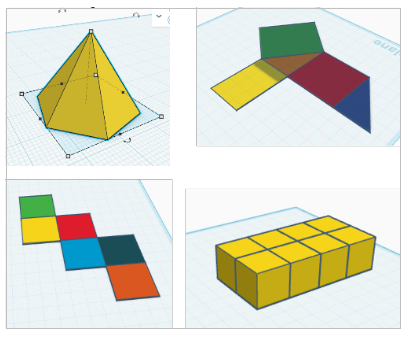
\includegraphics[width=0.4\textwidth]{images/bangun-dan-jaring.png}
            \caption{Desain 3D Bangun Ruang dan Jaring-jaring}
            \label{fig:bangundanjaring}
        \end{figure}
        \item Membuat Gambar Bangun Ruang dengan GeoGebra \\
        \hspace*{1cm}Gambar atau objek matematika yang terdapat dalam media ini sepenuhnya dibuat secara mandiri oleh peneliti. Objek-objek matematika, seperti persegi, kubus, balok, jaring-jaring, serta soal-soal, dibuat menggunakan aplikasi GeoGebra. Berikut ditampilkan contoh hasil pembuatannya.
        \begin{figure}[H]
            \centering
            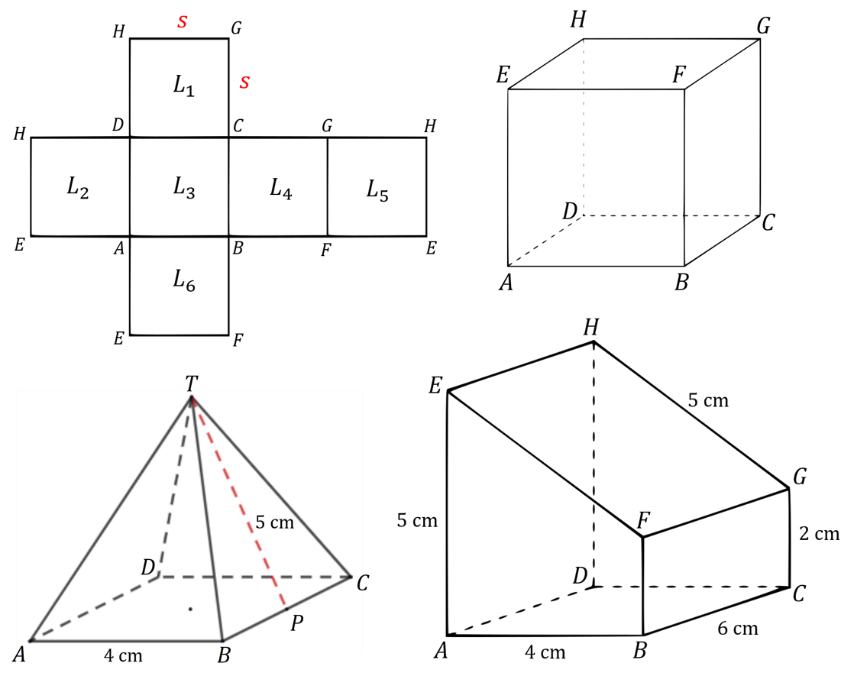
\includegraphics[width=0.4\textwidth]{images/hasil-geogebra.png}
            \caption{Desain 2D Bangun Ruang dan Jaring-jaring}
            \label{fig:hasilgeogebra}
        \end{figure}
        
        \item Membuat UI dengan React JS \\
        \hspace*{1cm}Agar media pembelajaran mudah diakses oleh peserta didik, peneliti membuat antarmuka menggunakan React JS. Antarmuka ini berbentuk situs web, sehingga peserta didik dapat dengan mudah mengakses media melalui domain yang diberikan. Untuk menampilkan simulasi 3D dan Augmented Reality di situs web, peneliti menggunakan Three.js sebagai paket tambahan serta mywebar.com untuk menampilkan konten AR. Berikut ditampilkan contoh hasil pembuatannya.
        \begin{figure}[H]
            \centering
            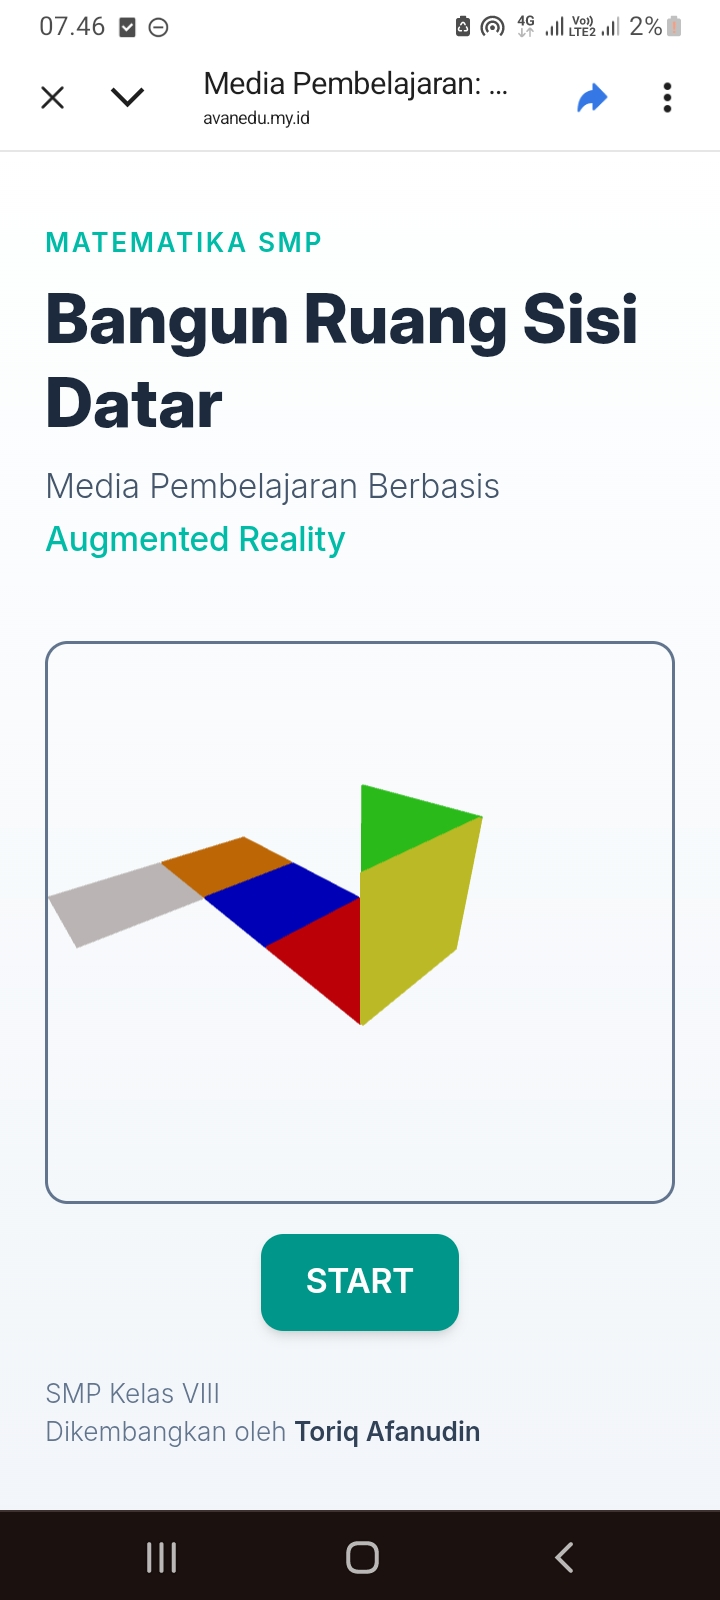
\includegraphics[width=0.3\textwidth]{images/ui-1.jpg}
            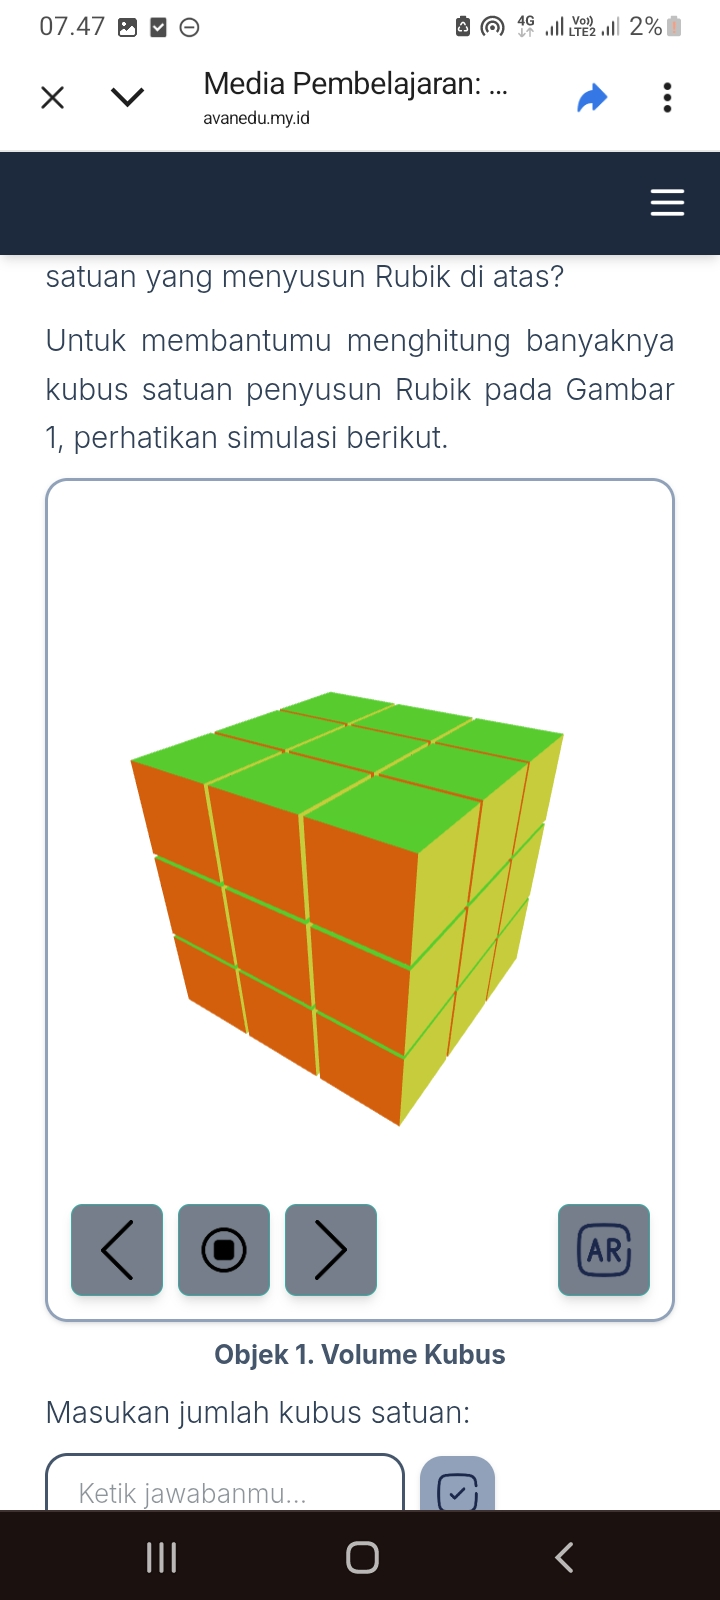
\includegraphics[width=0.3\textwidth]{images/ui-2.jpg}
            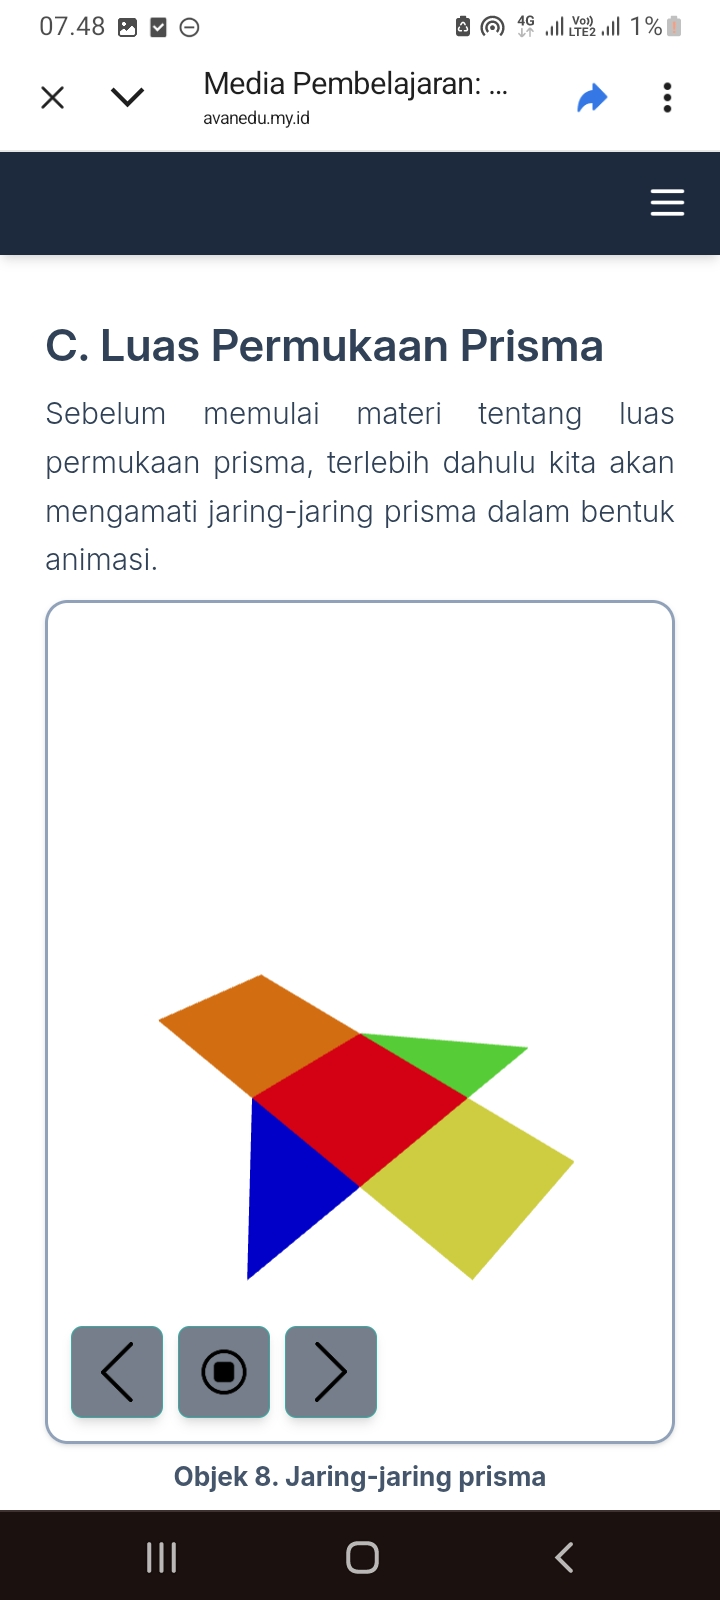
\includegraphics[width=0.3\textwidth]{images/ui-3.jpg}
            \caption{Antarmuka Media AR}
            \label{fig:antarmuka}
        \end{figure}

    \end{enumerate}

    \item \textbf{Implementasi}\\
    \hspace*{1cm}Pada tahap implementasi ini, peneliti melakukan uji coba terhadap produk yang telah dikembangkan. Uji coba dilakukan terhadap peserta didik kelas VIII-D SMP Negeri 3 Kalikajar. Tahap ini bertujuan untuk memperoleh informasi mengenai kelayakan media pembelajaran yang telah dikembangkan. Pada tahap ini, terdapat dua jenis uji coba yang dilakukan, yaitu uji coba kelas kecil dan uji coba kelas besar. Berikut adalah penjelasan mengenai uji coba kelas kecil dan uji coba kelas besar.
    \begin{enumerate}
        \item Uji Coba Kelas Kecil \\
        \hspace*{1cm}Uji coba kelas kecil dilakukan dengan melibatkan beberapa peserta didik dari kelas VIII-D. Pelaksanaan uji coba ini dilakukan melalui kegiatan pembelajaran menggunakan media pembelajaran yang sedang dikembangkan. Setelah pembelajaran selesai, peserta didik diminta mengisi angket untuk memperoleh informasi mengenai respons mereka terhadap media tersebut. Uji coba kelas kecil dilaksanakan pada tanggal 14 Mei 2024 dengan melibatkan 7 peserta didik kelas VIII-D yang dipilih secara acak.

        \hspace*{1cm}Pada tahap awal uji coba kelas kecil, peneliti terlebih dahulu meminta izin kepada pendidik matematika untuk melaksanakan uji coba terhadap 7 peserta didik kelas VIII-D. Pemilihan peserta didik dilakukan secara acak oleh pendidik matematika kelas VIII-D. Uji coba dilakukan dengan memberikan media pembelajaran dan angket kepada peserta didik. Angket tersebut digunakan untuk memperoleh data penilaian peserta didik terhadap media pembelajaran yang sedang dikembangkan. Hasil dari penyebaran angket dapat dilihat pada Tabel 3.

        \item Uji Coba Kelas Besar \\
        \hspace*{1cm}Uji coba kelas besar dilakukan dengan melibatkan seluruh peserta didik kelas VIII-D SMP Negeri 3 Kalikajar pada tanggal 16 Mei 2024. Pemilihan kelas tersebut didasarkan pada rekomendasi dari pendidik matematika. Alasan pemilihan ini adalah karena pendidik mengampu kelas tersebut dan peserta didik diketahui mengalami kesulitan dalam mempelajari materi bangun ruang.

        \hspace{1cm}Uji coba dilakukan melalui pembelajaran menggunakan media pembelajaran berbasis augmented reality. Setelah pembelajaran selesai, peserta didik diberikan angket. Angket tersebut digunakan untuk mengetahui penilaian peserta didik terhadap kualitas media pembelajaran yang dikembangkan. Pembelajaran dilaksanakan dengan membagi peserta didik ke dalam kelompok, disesuaikan dengan jumlah peserta didik yang membawa smartphone. Setelah peserta didik menyelesaikan materi dan soal-soal yang terdapat dalam media, mereka diminta untuk mengisi angket yang telah disediakan.
    \end{enumerate}

    \item \textbf{Evaluasi}
    
    \hspace{1cm}Tahap evaluasi merupakan tahap akhir dalam model pengembangan ADDIE. Evaluasi dilakukan untuk menganalisis hasil uji coba terhadap media pembelajaran berbasis augmented reality pada materi bangun ruang sisi datar kelas VIII. Tujuan dari tahap ini adalah untuk menyempurnakan produk yang telah dikembangkan sebelum menghasilkan produk akhir yang layak digunakan. Selanjutnya, dilakukan revisi akhir berdasarkan masukan dari ahli materi, ahli media, dan peserta didik.

    \hspace{1cm}Berdasarkan hasil validasi dari ahli materi dan ahli media, terdapat beberapa masukan terhadap media pembelajaran yang dikembangkan sebelum dilakukan uji coba kepada peserta didik. Selanjutnya, dilakukan revisi berdasarkan masukan tersebut hingga media pembelajaran masuk dalam kategori baik atau dinyatakan layak. Evaluasi yang dilakukan mencakup hasil validasi dari ahli materi dan ahli media, serta angket hasil uji coba media oleh peserta didik. Penilaian tersebut dijadikan acuan dalam menentukan kelayakan media pembelajaran yang dikembangkan.

\end{enumerate}
% ANALISIS DATA
\textbf{B. Analisis Data}

\hspace{1cm}Analisis data merupakan tahap lanjutan dari tahap evaluasi dalam model pengembangan ADDIE. Data yang diperoleh dalam penelitian ini berupa data kualitatif yang kemudian dikonversi menjadi data kuantitatif. Analisis data dilakukan berdasarkan lembar penilaian dari ahli materi, ahli media, dan respons peserta didik. Media pembelajaran yang dikembangkan dinyatakan layak apabila memperoleh skor rata-rata penilaian dari ahli materi, ahli media, dan respons peserta didik minimal pada kategori “baik”. Berikut ini adalah hasil analisis data tersebut:
\begin{enumerate}
    \item Analisis Penilaian Angket Ahli Materi\\
    \hspace*{1cm}Validasi oleh ahli materi dilakukan untuk memperoleh penilaian berupa skor, komentar, dan masukan terhadap materi yang telah dikembangkan dalam media pembelajaran berbasis augmented reality. Komentar dan saran dari validator digunakan untuk menyempurnakan media pembelajaran agar menghasilkan produk akhir yang layak digunakan. Kelayakan materi dalam media pembelajaran ini dinilai oleh dua orang ahli, yaitu Bapak Aan Hendroanto, M.Sc., dosen Pendidikan Matematika UAD, dan Ibu Wiwik Indarwati, S.Pd., pendidik Matematika di SMP Negeri 3 Kalikajar. Hasil penilaian kelayakan media pembelajaran disajikan pada Tabel \ref{penilaianmateri}.
    \begin{table}[H]
        \begin{adjustwidth}{-2cm}{-2cm}
            \centering
            \caption{Hasil Penilaian Media Pembelajaran Menurut Ahli Media}
            \label{penilaianmateri}
            \begin{tabular}{|c|c|c|c|c|c|}
                \hline
                \textbf{No} & \textbf{Validator} & \textbf{Skor} & \textbf{Rata-rata Skor} & \textbf{Kriteria Data Kuantitatif}\\
                \hline
                1 & Aan Hendroanto, M.Sc. & 0 & 0 & Sangat Baik\\
                2 & Wiwik Indarwati, S.Pd. & 0 & 0 & Sangat Baik\\
                \hline
                \multicolumn{2}{|c|}{Jumlah Skor} & 0 & & \\
                \hline
                \multicolumn{2}{|c|}{Rata-rata Keseluruhan} & 0 & 0 & Sangat Baik\\
                \hline
            \end{tabular}
        \end{adjustwidth}
    \end{table}

    \begin{table}[H]
        \centering
        \caption{Kriteria Penilaian Ahli Materi}
        \begin{tabular}{|c|c|c|}
            \hline
            \textbf{No} & \textbf{Rentang Skor \( (i) \) Kuantitatif} & \textbf{Kategori Kualitatif}\\
            \hline
            1 & \( \bar{x} > 4{,}21 \) & Sangat Baik\\
            2 & \( 3{,}41 < \bar{x} \leq 4{,}2 \) & Baik\\
            3 & \( 2{,}60 < \bar{x} \leq 3{,}41 \) & Cukup Baik\\
            4 & \( 1{,}80 < \bar{x} \leq 2{,}60 \) & Kurang\\
            5 & \( \bar{x} \leq 1{,80} \) & Sangat Kurang\\
            \hline 
        \end{tabular}
    \end{table}

    \item Analisis Penilaian Angket Ahli Media\\
    \hspace*{1cm}Validasi oleh ahli media dilakukan untuk memperoleh penilaian berupa skor, komentar, dan masukan terhadap media pembelajaran yang dikembangkan. Komentar dan saran dari validator media digunakan untuk menyempurnakan media pembelajaran agar menghasilkan produk akhir yang layak digunakan. Kelayakan media pembelajaran ini dinilai oleh dua orang ahli media, yaitu Bapak Anggit Prabowo, M.Pd., dosen Pendidikan Matematika UAD, dan Ibu Wiwik Indarwati, S.Pd., pendidik Matematika di SMP Negeri 3 Kalikajar. Hasil penilaian kelayakan oleh ahli media disajikan pada Tabel~\ref{penilaianmedia}.
    \begin{table}[H]
        \begin{adjustwidth}{-2cm}{-2cm}
            \centering
            \caption{Hasil Penilaian Media Pembelajaran Menurut Ahli Media}
            \label{penilaianmedia}
            \begin{tabular}{|c|c|c|c|c|c|}
                \hline
                \textbf{No} & \textbf{Validator} & \textbf{Skor} & \textbf{Rata-rata Skor} & \textbf{Kriteria Data Kuantitatif}\\
                \hline
                1 & Anggit Prabowo, M.Pd. & 0 & 0 & Sangat Baik\\
                2 & Wiwik Indarwati, S.Pd. & 0 & 0 & Sangat Baik\\
                \hline
                \multicolumn{2}{|c|}{Jumlah Skor} & 0 & & \\
                \hline
                \multicolumn{2}{|c|}{Rata-rata Keseluruhan} & 0 & 0 & Sangat Baik\\
                \hline
            \end{tabular}
        \end{adjustwidth}
    \end{table}

    \begin{table}[H]
        \centering
        \caption{Kriteria Penilaian Ahli Media}
        \begin{tabular}{|c|c|c|}
            \hline
            \textbf{No} & \textbf{Rentang Skor \( (i) \) Kuantitatif} & \textbf{Kategori Kualitatif}\\
            \hline
            1 & \( \bar{x} > 4{,}21 \) & Sangat Baik\\
            2 & \( 3{,}41 < \bar{x} \leq 4{,}2 \) & Baik\\
            3 & \( 2{,}60 < \bar{x} \leq 3{,}41 \) & Cukup Baik\\
            4 & \( 1{,}80 < \bar{x} \leq 2{,}60 \) & Kurang\\
            5 & \( \bar{x} \leq 1{,80} \) & Sangat Kurang\\
            \hline 
        \end{tabular}
    \end{table}

    \item Analisis Penilaian Angket Respons Peserta Didik\\
    \hspace*{1cm}Respons peserta didik diperoleh melalui uji coba kelas kecil dan uji coba kelas besar yang bertujuan untuk mendapatkan penilaian berupa skor, komentar, dan masukan terhadap media pembelajaran yang telah dikembangkan. Respons tersebut dianalisis berdasarkan hasil angket yang disebarkan kepada peserta didik kelas VIII-D SMP Negeri 3 Kalikajar. Kriteria penilaian angket respons peserta didik disajikan pada Tabel \ref{kriteriaresponsiswa}.
    \begin{table}[H]
        \centering
        \caption{Kriteria Penilaian Respon Peserta Didik}
        \label{kriteriaresponsiswa}
        \begin{tabular}{|c|c|c|}
            \hline
            \textbf{No} & \textbf{Rentang Skor \( (i) \) Kuantitatif} & \textbf{Kategori Kualitatif}\\
            \hline
            1 & \( \bar{x} > 4{,}21 \) & Sangat Baik\\
            2 & \( 3{,}41 < \bar{x} \leq 4{,}2 \) & Baik\\
            3 & \( 2{,}60 < \bar{x} \leq 3{,}41 \) & Cukup Baik\\
            4 & \( 1{,}80 < \bar{x} \leq 2{,}60 \) & Kurang\\
            5 & \( \bar{x} \leq 1{,80} \) & Sangat Kurang\\
            \hline 
        \end{tabular}
    \end{table}
    \item Kualitas Produk Secara Keseluruhan\\
    \hspace*{1cm}Kualitas media pembelajaran secara keseluruhan dinilai berdasarkan skor rata-rata dari ahli materi, ahli media, uji coba kelas kecil, dan uji coba kelas besar. Hasil perhitungan rata-rata keseluruhan dari keempat penilaian tersebut disajikan pada Tabel~\ref{ratakeseluruhan}.\\
    \begin{table}[H]
        \centering
        \caption{Hasil Rata-rata Keseluruhan}
        \label{ratakeseluruhan}
        \begin{tabular}{|c|c|c|c|}
            \hline
            \textbf{No} & \textbf{Sampel Uji Coba} & \textbf{Rata-rata} & \textbf{Kriteria}\\
            \hline
            1 & Ahli Materi & 0 & Sangat Baik\\
            2 & Ahli Media & 0 & Sangat Baik\\
            3 & Uji Coba Kelas Kecil & 0 & Sangat Baik\\
            4 & Uji Coba Kelas Besar & 0 & Sangat Baik\\
            \hline
            \multicolumn{2}{|c|}{Rata-rata Keseluruhan} & 0 & Sangat Baik\\
            \hline
            
        \end{tabular}
    \end{table}
    \hspace*{1cm}Berdasarkan Tabel~\ref{ratakeseluruhan}, terlihat bahwa hasil perhitungan rata-rata secara keseluruhan dari ahli materi, ahli media, uji coba kelas kecil, dan uji coba kelas besar memperoleh skor rata-rata sebesar XXX dan termasuk dalam kategori sangat baik. Dengan demikian, media pembelajaran berbasis augmented reality yang dikembangkan dinyatakan layak untuk digunakan.

\end{enumerate}
% REVISI PRODUK
\textbf{C. Revisi Produk}

\hspace*{1cm}Revisi produk merupakan langkah penting dalam pengembangan media pembelajaran. Revisi dilakukan apabila masih terdapat kesalahan atau kekurangan pada produk yang dikembangkan. Pada tahap ini, peneliti melakukan revisi terhadap media pembelajaran berdasarkan saran dan masukan dari ahli materi dan ahli media. Adapun proses revisi dalam pengembangan media pembelajaran ini adalah sebagai berikut:
\begin{enumerate}
    \item Revisi Produk Hasil Validasi Ahli Materi\\
    \hspace*{1cm}Berdasarkan masukan dari ahli materi, perbaikan yang dilakukan telah sesuai dengan saran dan rekomendasi yang diberikan. Hasil perbaikan tersebut disajikan sebagai berikut.
    \begin{enumerate}
        \item Menambahkan kelas dan logo UAD pada halaman sampul.
        \item Menambahkan ilustrasi kubus satuan yang tidak dapat dihitung menggunakan tombol.
        \item Menyisipkan teknologi AR pada soal, tidak hanya pada materi.
        \item Menambahkan materi mengenai unsur-unsur bangun ruang.
        \item Memperbaiki penggunaan tanda baca pada kalimat-kalimat dalam media.
    \end{enumerate}
    \item Revisi Produk Hasil Validasi Ahli Media
    \item Revisi Produk Hasil Uji Coba Kelas Kecil
    \item Revisi Produk Hasil Uji Coba Kelas Besar
\end{enumerate}

\textbf{D. Kajian Produk Akhir}

\hspace*{1cm}Media pembelajaran yang dikembangkan oleh peneliti disusun dengan isi sebagai berikut:
\begin{enumerate}
    \item Halaman Sampul\\
    \hspace*{1cm}Halaman ini menampilkan judul, judul materi, sasaran, serta nama pengembang.
    \begin{figure}[H]
        \centering
        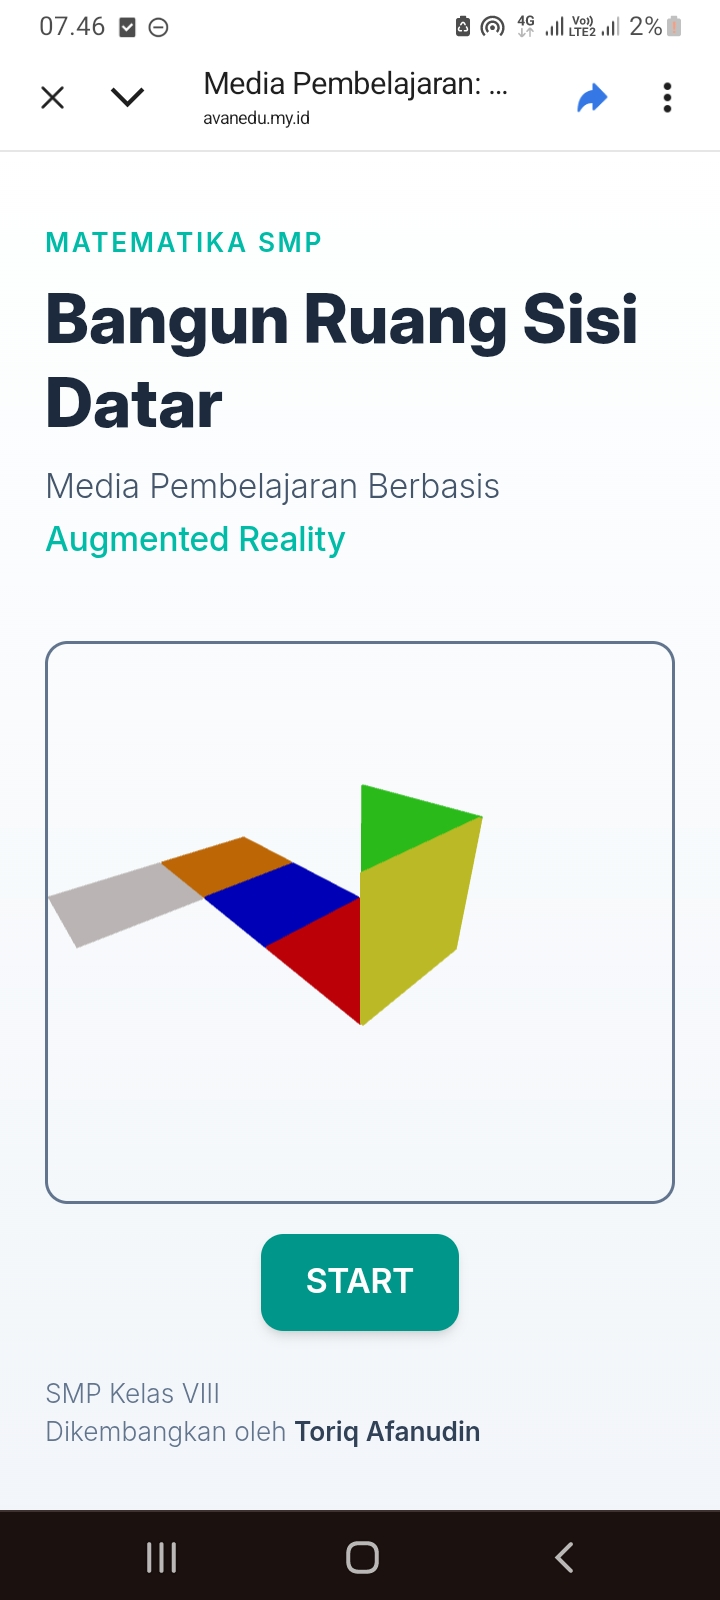
\includegraphics[width=0.3\textwidth]{images/ui-1.jpg}
        \caption{Halaman Sampul}
        \label{fig:sampul}
    \end{figure}
    \item Halaman Petunjuk\\
    \hspace*{1cm}Pada halaman ini, peserta didik dapat mengunduh barcode yang dibutuhkan untuk menampilkan augmented reality (AR) serta berlatih menggunakan AR sebelum memulai pembelajaran.
    \begin{figure}[H]
        \centering
        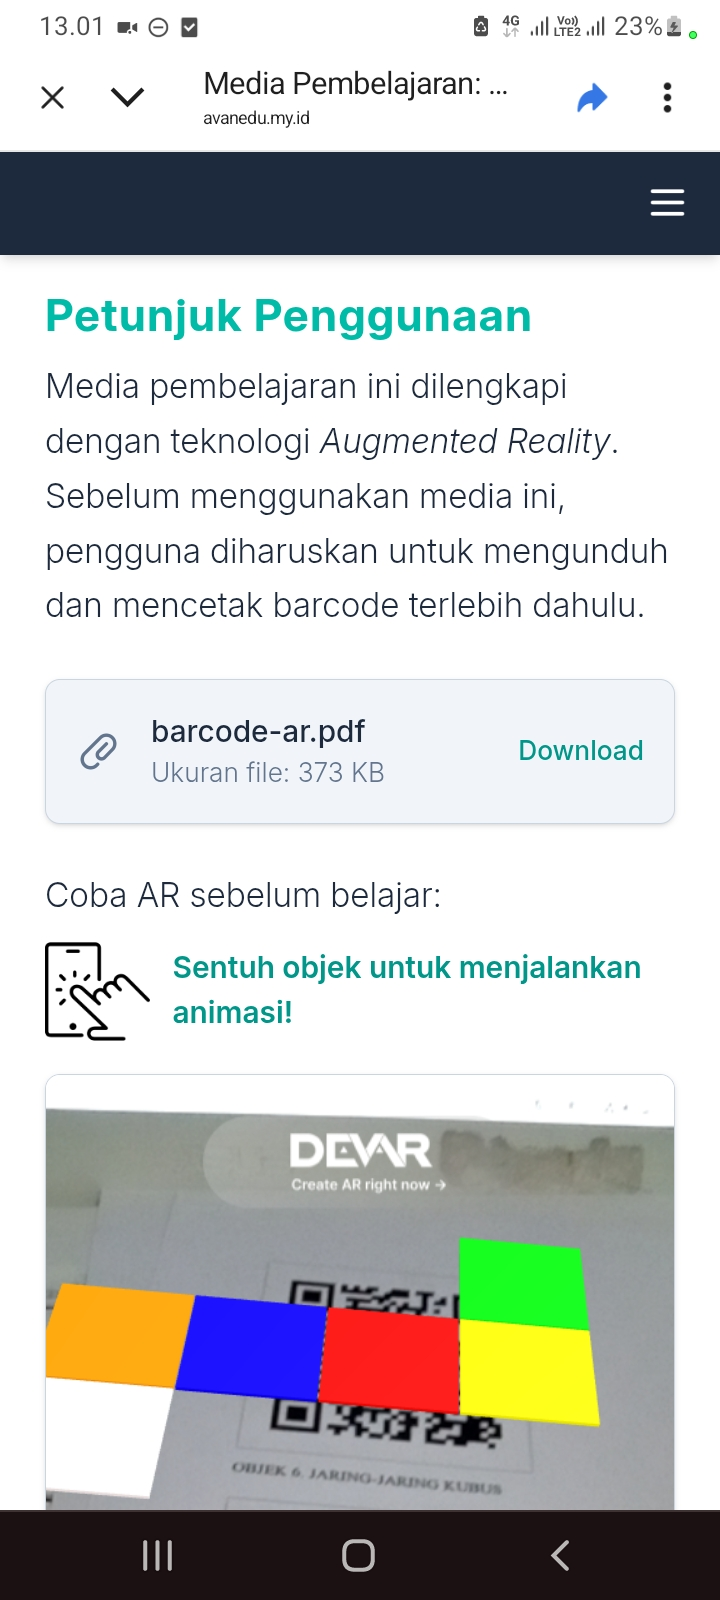
\includegraphics[width=0.25\textwidth]{images/petunjuk.jpg}
        \caption{Halaman Petunjuk}
        \label{fig:petunjuk}
    \end{figure}
    \item Halaman Menu\\
    \hspace*{1cm}Pada halaman ini, peserta didik dapat memilih materi yang ingin dipelajari atau langsung mengerjakan kuis.
    \begin{figure}[H]
        \centering
        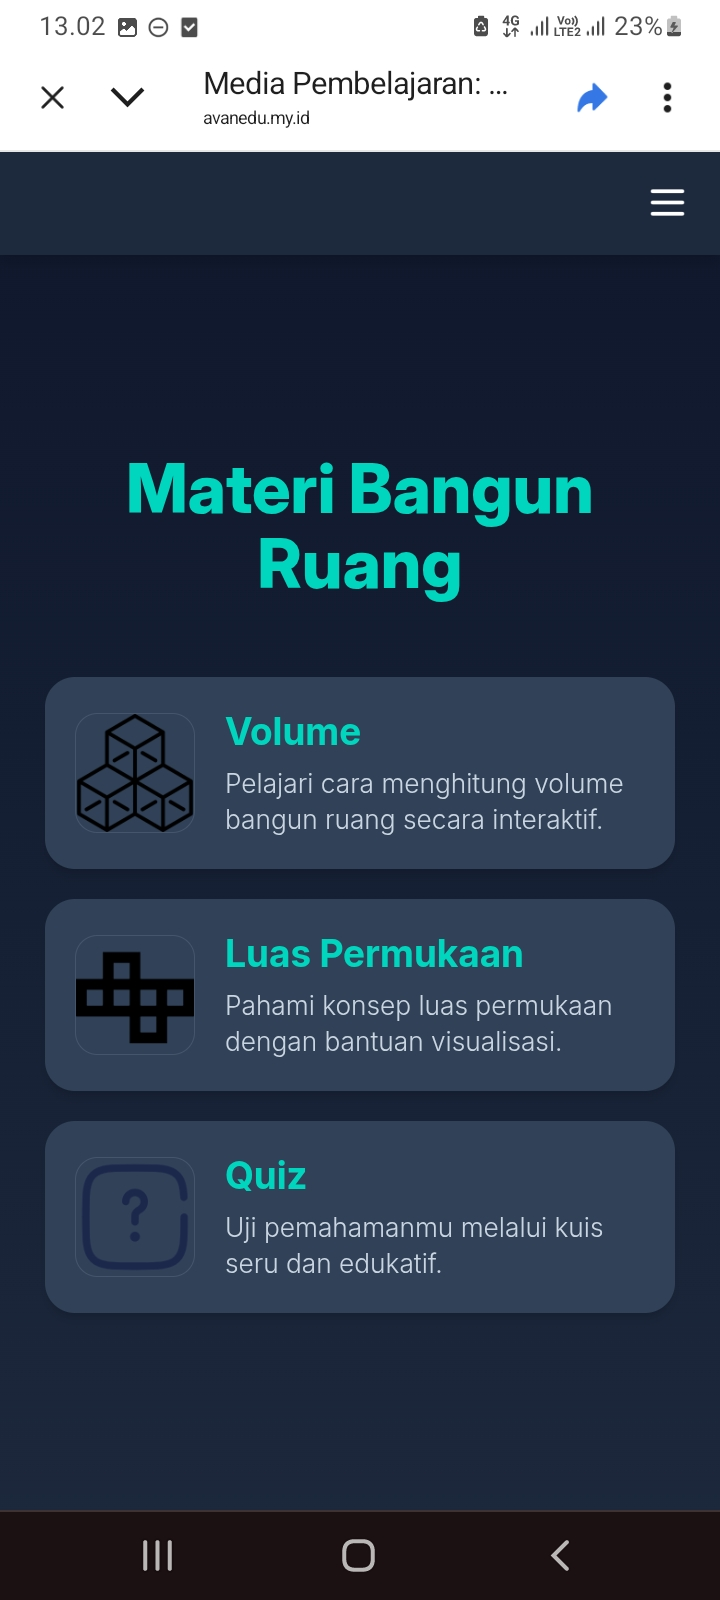
\includegraphics[width=0.2\textwidth]{images/menu.jpg}
        \caption{Halaman Menu}
        \label{fig:menu}
    \end{figure}

    \item Halaman Materi\\
    \hspace*{1cm}Pada halaman materi, peserta didik akan mempelajari dua topik utama, yaitu volume dan luas permukaan bangun ruang. Peserta didik akan melihat bangun ruang yang disajikan dalam bentuk 3D dan augmented reality. Bangun ruang tersebut juga dapat dianimasikan untuk mempermudah pemahaman. Untuk mengevaluasi pemahaman peserta didik, tersedia latihan soal di akhir setiap bab.
    \begin{figure}[H]
        \centering
        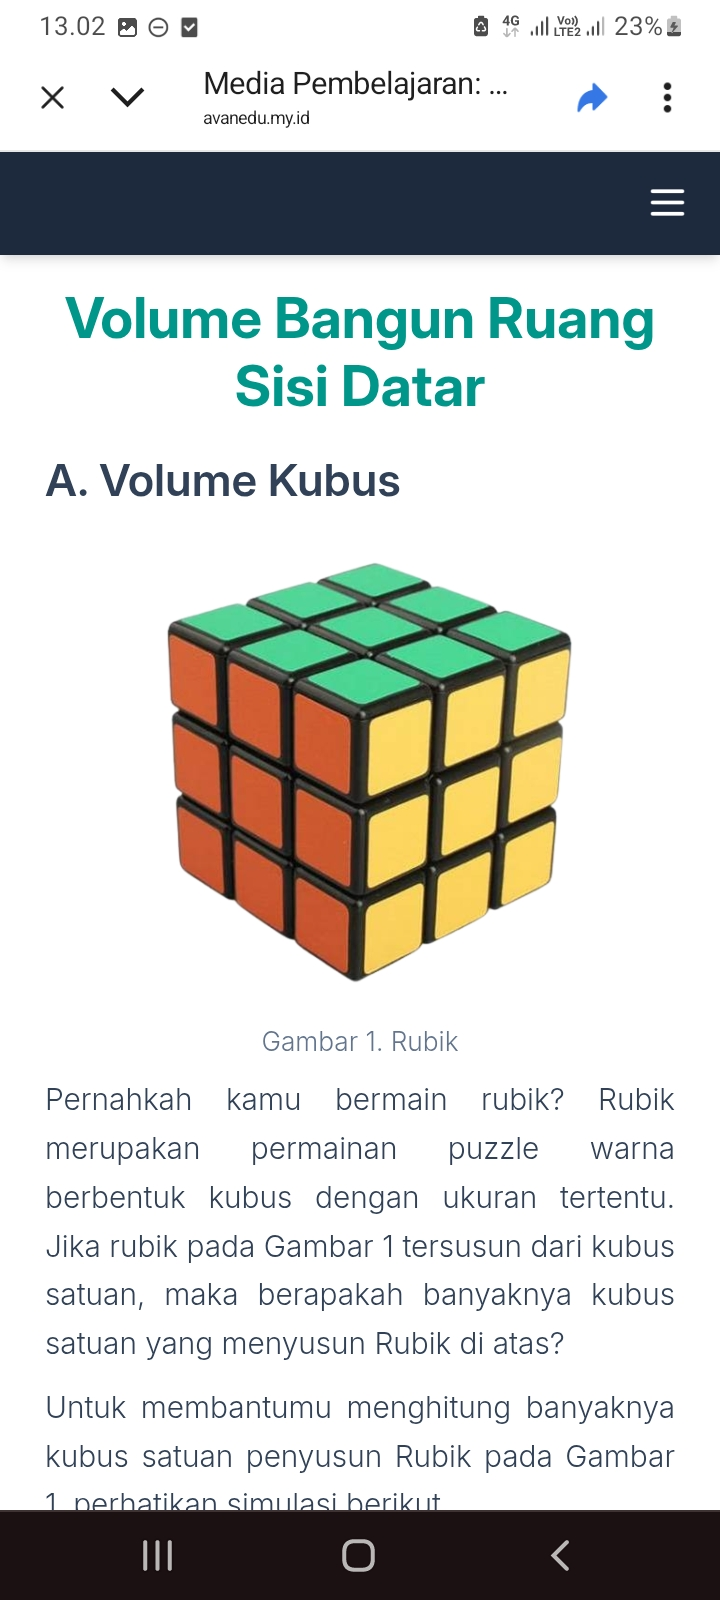
\includegraphics[width=0.2\textwidth]{images/materi1.jpg}
        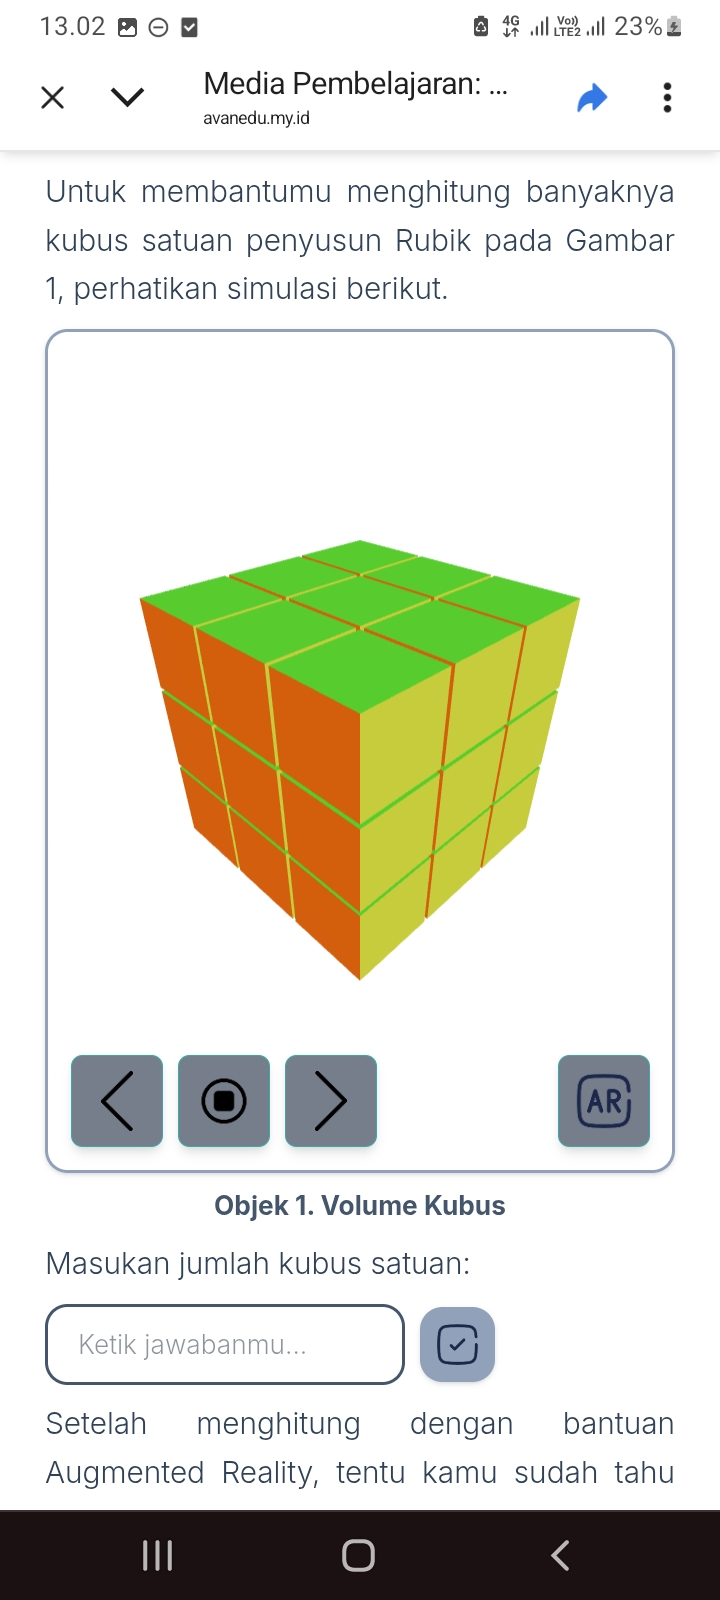
\includegraphics[width=0.2\textwidth]{images/materi2.jpg}
        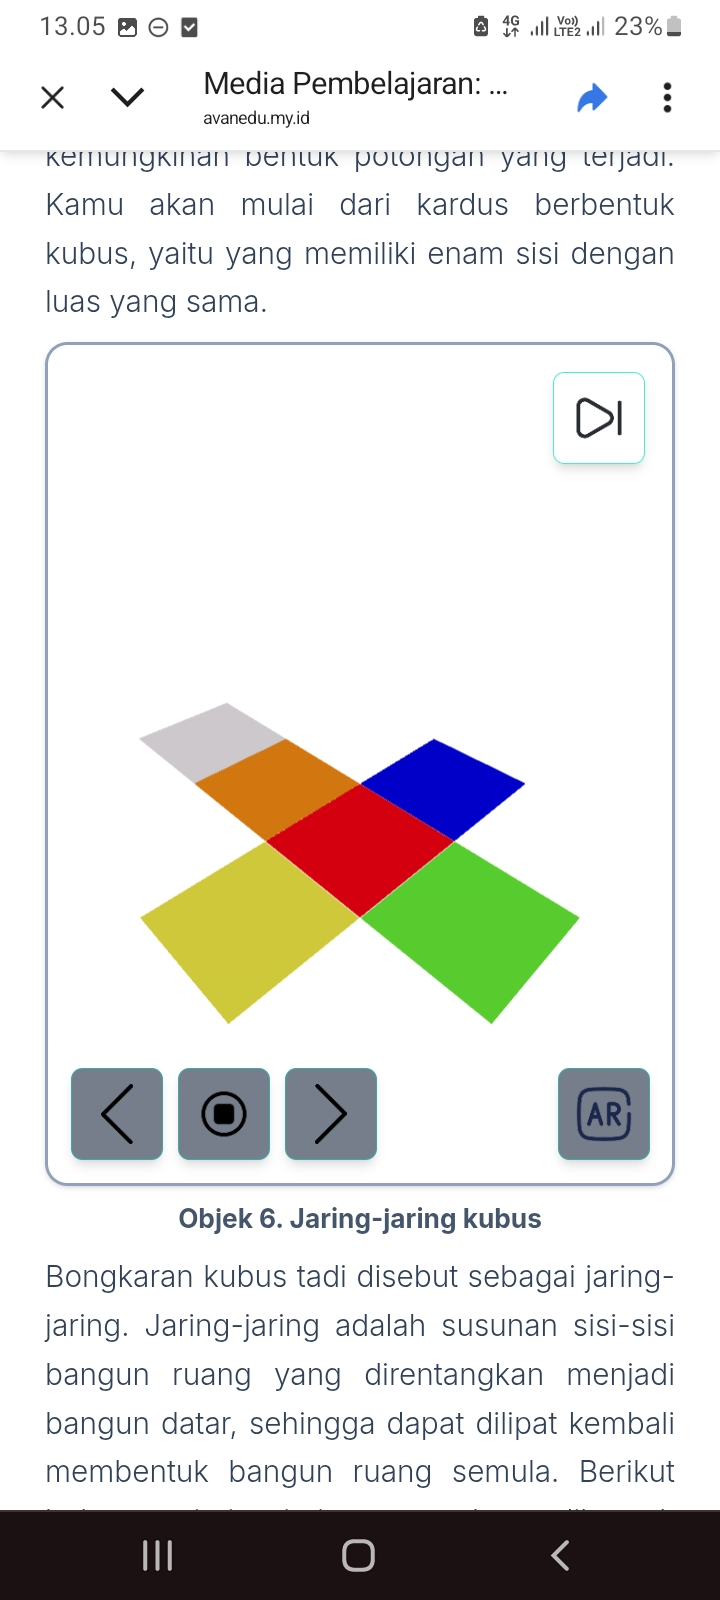
\includegraphics[width=0.2\textwidth]{images/materi3.jpg}
        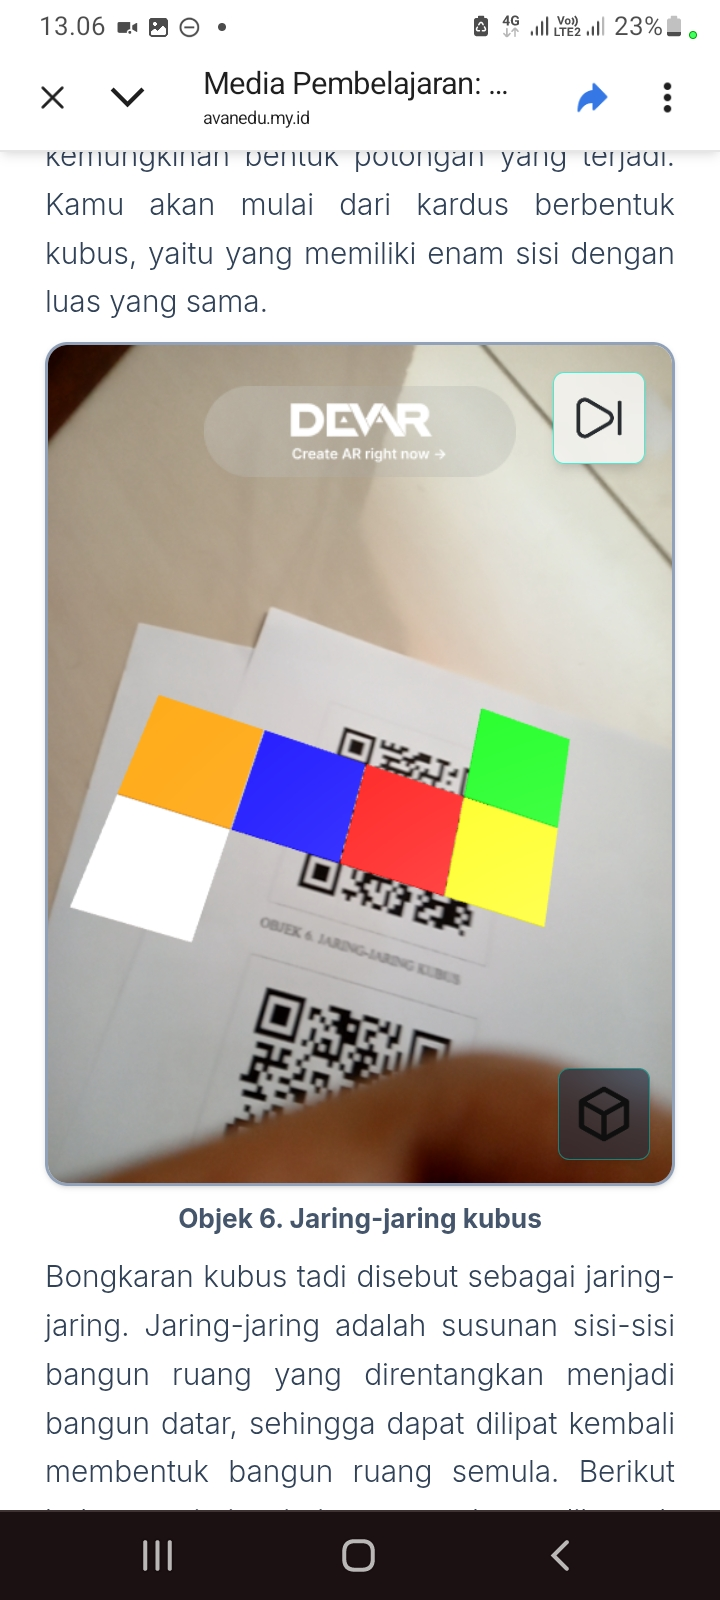
\includegraphics[width=0.2\textwidth]{images/materi4.jpg}
        \caption{Halaman Materi}
        \label{fig:materi}
    \end{figure}

    \item Halaman Kuis\\
    \hspace*{1cm}Pada halaman kuis, disajikan lima soal yang sesuai dengan latihan soal di akhir setiap bab. Terdapat juga penghitung waktu (timer) dengan batas waktu pengerjaan selama 30 menit. Untuk mulai mengerjakan kuis, peserta didik perlu memasukkan kode ujian. Peserta didik dapat menjawab soal dengan mengisi kolom jawaban yang disediakan, serta dapat menyisipkan foto untuk memperkuat jawabannya.

\end{enumerate}


\end{document}
